\subsection{Detection Probabilities}
At this stage, the drawing of GRB properties according to the specified 
functions
and the subsequent derivation and calculation of the signal expectation in
IceCube has been explained. However, the Optical (and X-ray) Follow-Up does not
trigger on singlets but on multiplets fulfilling several criteria.

Multiplets are a number of neutrinos that arrive within 100 s and 3.5 degrees
of each other (chapter \ref{sec:OFU_alert_system}). A test statistic was 
implemented to select the
most signal like doublets to trigger Swift Follow-Up observations. Once 
triggered there
is a chance that a source will not be within the FoV of the XRT. The 
probabilities for two neutrinos to pass these criteria will be 
explained in this section.

\subsubsection{Doublet Probabilities}

\paragraph{Probability to detect two neutrinos $P_{2 \nu}$}$\;$\\
In section \ref{subsubsec:NExp}, the number of expected neutrinos per 
GRB $\mu$ was calculated. 
Given this number, the probability to see $N$ neutrinos is given with the 
Poisson 
distribution
\begin{equation}
  P_\text{Poisson}(N, \mu) = \frac{\mu^N}{N!} \exp^{-\mu}
\end{equation}
Hence, the probability to see exactly one neutrino and one or more neutrinos is 
\begin{eqnarray}
 P_{1 \nu} &= P_\text{Poisson}(1, \mu) \\
 P_{\geq 1 \nu} &= 1 - P_\text{Poisson}(0, \mu)
\end{eqnarray}
The subsequent probabilities apply to the case of exactly two detected 
neutrinos.
\begin{equation}
 P_{2\nu} = P_\text{Poisson}(2, \mu) = \frac{\mu^2}{2!} \exp^{-\mu}
\end{equation}


\paragraph{P$_{\Delta t}$}$\;$\\
% \\
%  \Rightarrow \tau &= \frac{-t_{90}}{\text{ln}(0.1)}
P$_{\Delta t}$ is the probability that two neutrinos arrive within
100 seconds, the time window
specified in the doublet search. 
It decreases exponentially with time if the lightcurve is assumed to be fast 
rising
with an exponential decay (FRED)
\begin{equation}
 P(\Delta t) = 1 - e^{\left(-\frac{\Delta t}{\tau} \right)}.
\end{equation}
$\tau$ can be determined according to equation \ref{eq:ToyMC_tau} given
a specific $t_{90}$ (drawn according to \ref{eq:t90dist} and converted in 
agreement
with \ref{eq:t90earth}). For the Optical Follow-Up
$\Delta t_{max} =100 \text{ s}$ is currently set. 
%more detail here? too much just refering to other equations?
The effects of different time
windows could be examined by choosing different values. However, this is not
the focus of this work.



\paragraph{P$_{3.5^\circ}$}$\;$\\
The second requirement for each neutrino pair is that they arrive with a
maximum angular separation of 3.5 degrees. To calculate this probability 
P$_{3.5^\circ}$ for a given GRB, NuGen events need to be
selected from within the zenith band (chapter \ref{sec:zenith_bands}) and
shifted to the GRB direction (chapter \ref{sec:shift2source}). 
% Each remaining event is paired with all other events, 
To save on computation time, 4000 of the NuGen events are selected randomly
and the angular 
differences of the
shifted reconstructed directions are determined for each event combination. The 
probability is then the
ratio between the sum of the weight products (term $i$ and $j$ in Eq. 
\ref{eqn:Nexp_wZB_wEps}) of
all event pairs passing the $3.5^\circ$ cut and all evaluated pairs
\begin{equation}
\label{eq:P3p5}
 P_{3.5^\circ} = \frac{\sum_{i} \sum_{j=i+1} w_i \cdot w_j | \Delta \Psi(i, j)
\leq
3.5^{\circ}}{\sum_i \sum_{j=i+1} w_i \cdot w_j}
\end{equation}
Though selecting 4000 events randomly speeds up this calculation, combining 
each event of the selection with all others requires computational power 
and time. 
If all events from within the zenith bands were to be considered, all events 
and therefore the probability $P_{3.5^\circ}$ should be the same for all GRBs 
coming from the exact same zenith angle suggesting that a parameterization in 
dependence of the drawn GRB zenith angle should be possible. 

About 8000 GRBs are drawn for each season and HESE spectra
%  and GRB model 
and the probability calculated according to \ref{eq:P3p5}. The resulting 
parameterization 
$P_{3.5^\circ}(\theta_\text{GRB})$ is then used to simulate GRBs in greater 
numbers.
Exemplary, two cases are shown here to demonstrate the quality and the 
different behavior of the parameterization in different seasons.

The probabilities follow different behaviors in different zenith ranges. Using 
a 
hard spectrum with $\gamma=2$ and the NuGen dataset of the BDT season, the 
probability is displayed  vs
$\theta_\text{GRB}$ in a 2d histogram in Fig. \ref{fig:P3p5param_bdt_gamma2}. A 
mean probability value is calculated for each $\theta_\text{GRB}$ bin.
The probability follows two different functional behaviors. A hyperbolic 
tangent is fitted to the data near the pole ($\cos(\theta_\text{GRB}) 
\leq -0.81$)
\begin{equation}
\label{eq:Ptanh}
 P = a \cdot \text{tanh}(b \cdot (\cos(\theta_\text{GRB}- c)) + d
\end{equation}
while a simple polynomial function of the fifth order is used in the second 
region
\begin{equation}
\label{eq:PPoly}
 P = a \cdot \cos^5\theta_\text{GRB} + b \cdot 
\cos^4\theta_\text{GRB} + c \cdot \cos^3\theta_\text{GRB} + d 
\cdot \cos^2\theta_\text{GRB} + e \cdot \cos\theta_\text{GRB} + f
\end{equation}
Next to the mean probability of each bin, the fits use the coordinates of 
the mean of these averaged values between the 
last bin of the first region and the first bin of the last region and the 
splitting zenith value as an additional data point.
The quality of the parameterization was examined by creating a second dataset 
of GRBs. The probability was calculated according to Eq. 
\ref{eq:P3p5} based on all 
NuGen events within a zenith region around a GRB ($P_{3.5^\circ}^\text{MC}$) 
and parametrized according to the fit to the first 
dataset ($P_{3.5^\circ}^\text{param}$).
% to characterize the probability with the most 
% information available.
A good agreement between the two procedures is presented in Fig. 
\ref{fig:P3p5param_bdt_gamma2_quality} with a maximum deviation of about 1\%.

\begin{figure}[h]
\centering
 \captionsetup{width=.9\textwidth}
\subfloat[Parametrization (blue line) of the 
probability $P_{3.5^\circ}$\label{fig:P3p5param_bdt_gamma2}]{%
  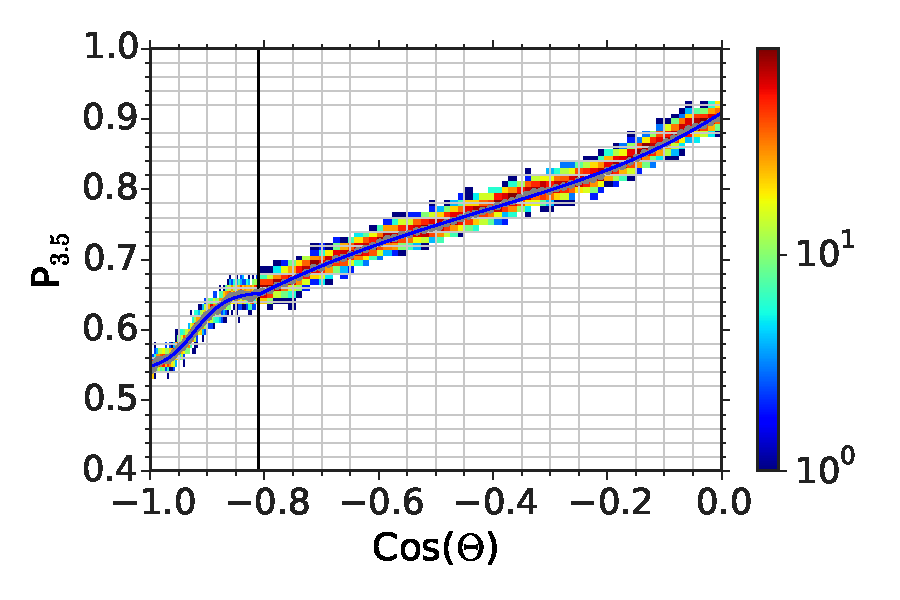
\includegraphics[width=0.45\textwidth]{fig/P3p5param_bdt_gamma2.pdf}}
\subfloat[Testing the 
parameterization with a second 
dataset.\label{fig:P3p5param_bdt_gamma2_quality}]{%
  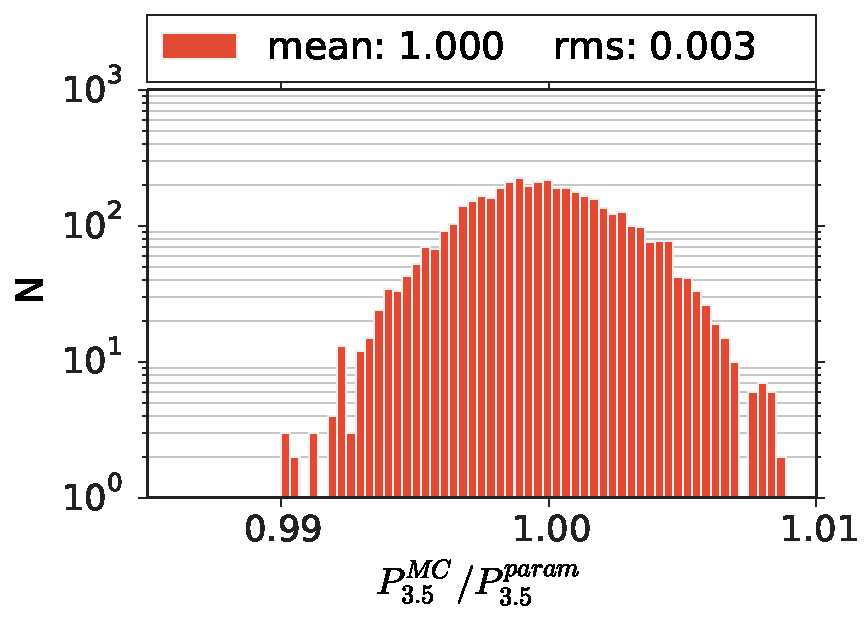
\includegraphics[width=0.45\textwidth]{fig/P3p5param_bdt_gamma2_quality.pdf}}
\caption{IC86-BDT season: The probability of neutrino events to be within 3.5\% 
of each other and the dependency on the cosinus of the GRB zenith angle. The 
blue line represents the parameterization (left). Using a second set of 
simulated GRBs, a histogram 
of the ratio between the calculated probabilities based on all events in 
the zenith bands and the parametrized values is shown (right). The maximum 
deviation 
is about 1\%.}
\end{figure}

The second example (IC86-2) demonstrates the difference between the IC86-1/2 
seasons 
and the BDT season. The dependence of the zenith angle shows more structure 
(Fig \ref{fig:P3p5param_862_gamma2}) and the parameterization is split into 
four regions. The data in the first one starting at the pole is fitted with a
hyperbolic tangent (Eq. \ref{eq:Ptanh}) while the data in the other three 
regions are all fitted with the polynomial function (Eq. \ref{eq:PPoly}) each.

\begin{figure}[h]
\centering
 \captionsetup{width=.9\textwidth}
%  \captionsetup{margin=0pt}
 \subfloat[Parametrization (blue line) of the 
probability $P_{3.5^\circ}$\label{fig:P3p5param_862_gamma2}]{%
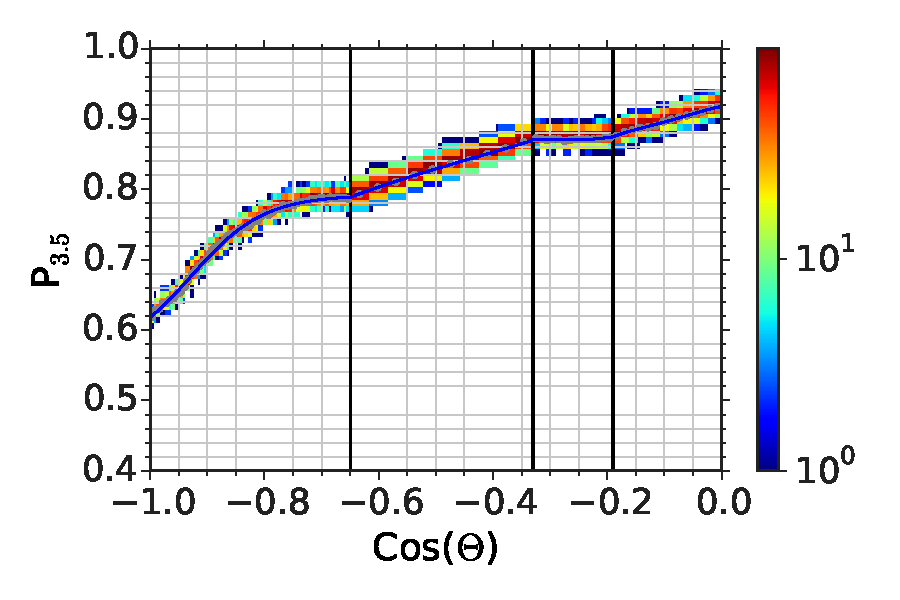
\includegraphics[width=0.45\textwidth]{fig/P3p5param_862_gamma2.pdf}}
\subfloat[Testing the 
parameterization with a second 
dataset.\label{fig:P3p5param_862_gamma2_quality}]{%
 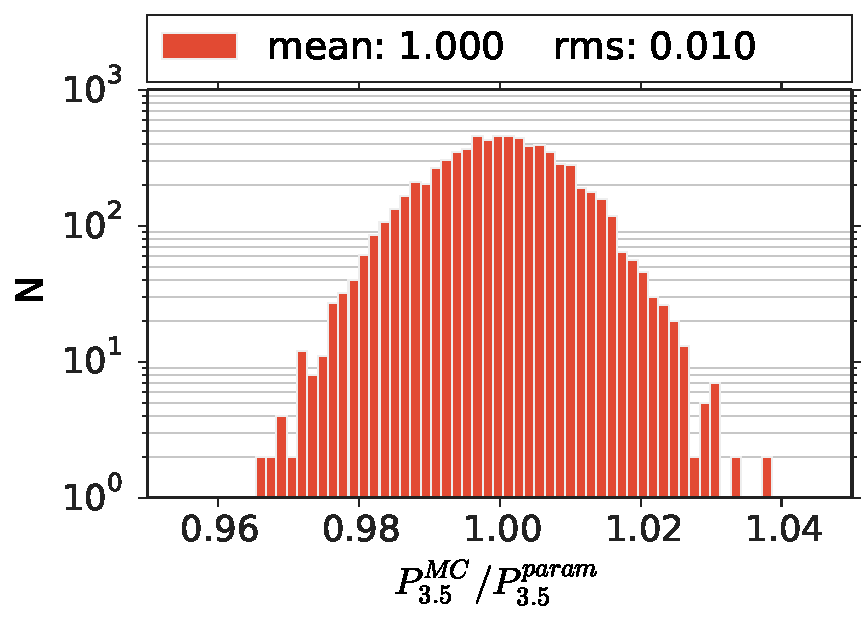
\includegraphics[width=0.45\textwidth]{fig/P3p5param_862_gamma2_quality.pdf}}
\caption{IC86-2 season: The probability of neutrino events to be within 3.5\% 
of each other and the dependency on the cosinus of the GRB zenith angle. The 
blue line represents the parameterization (left). Using a second set of 
simulated GRBs, a histogram 
of the ratio between the calculated probabilities based on all events in 
the zenith bands and the parametrized values is shown (right). The maximum 
deviation 
is about 4\%.}
\end{figure}
The quality of the parameterization can be examined in Fig. 
\ref{fig:P3p5param_862_gamma2_quality}. The overall result is still very 
satisfying though the root mean square is with 0.01 instead of 0.003 larger as 
is the maximum deviation of about 4\% instead of 1\%. However, the 
probabilities $P_{3.5^\circ}^\text{MC}$ in the second control dataset are 
not based on all events within the zenith region in this test. Instead, a 
random selection of 4000 events was used as well leading to possible 
fluctuations of the comparison points compared to the optimal value based on all 
events.
% enabling the comparison of the 
% parametrized value to a deviation of the optimal value based on all events. 
Thus, the slightly worse but still good result is explained and the 
parameterization will be used.

The final probability per zenith direction is not dependent on the absolute 
normalization of the flux as it cancels in equation \ref{eq:P3p5}, but on the 
chosen OFU cuts and the spectral shape. The season and the signal spectrum
define the amount 
events of different energies contribute to the calculation. Therefore, the 
probability is parametrized once per season and spectral index $\gamma$ and is 
then used for all GRB models. The root-mean-square suffers by about 0.1 - 0.2 
percentage points in comparison to individual parameterizations per season, 
$\gamma$ and GRB model and is considered acceptable.

The fitted values to the free parameters in Eq. \ref{eq:Ptanh} and 
\ref{eq:PPoly} as well as the break points between the different regions are 
listed for all season - spectra combinations in table \ref{tab:P3p5fitvalues}.

\begin{table}[h]
  \centering
  \begin{tabular}{r|c|r||l|l|r|l|l|l|l}
season  &  $\gamma$ & region & $b_i$ & a & b & c 
& d & e & f \\
\hline\hline
IC86-1 & 2 & I & -1 &0.113& 7.847& -0.923 &  0.680& - & 
-\\
IC86-1 & 2 & II & -0.65 & 1.206 & 2.472 & 7.126 & 9.782 & 
4.855 \\
IC86-1 & 2 & III & -0.33 & 3.257e-02 & -1.455e+01 & -9.1460e+01 
& -2.488e+02 & -2.481e+02 \\
IC86-1 & 2 & IV & -0.21 & 9.198e-01 & 3.415e-02 & -3.649e+00 &  
-2.404e+01 & -5.053e+01 \\
\hline
IC86-2 & 2 & I &  -1 & 0.115 & 7.857 & -0.928 & 0.678 & - 
& -\\
IC86-2 & 2 & II & -0.65 & 1.041 & 0.910 & 2.191 & 2.687 & 
1.140 \\
IC86-2 & 2 & III &  -0.33 & 0.753 & -2.582 & -18.718 & 
-56.052 &  -59.955 \\
IC86-2 & 2 & IV &  -0.19 & 0.918 & 0.156 & -1.679 & 
-14.0167 & -37.505 \\
\hline
IC86-BDT & 2 & I & -1 & 0.056 & 17.705 & -0.923 & 0.598 & - & - 
\\
IC86-BDT & 2 & II & -0.81 & 0.909 & 0.525 & 0.728 & 0.724 & 0.171 \\
\hline
\hline
IC86-1 & 2.3 & I & -1 & 0.121 & 8.142 & -0.915 & 0.649 & - & -\\
IC86-1 & 2.3 & II & -0.66 & 0.699 & -1.484 & -4.571 & -5.137 & -2.116 \\
IC86-1 & 2.3 & III & -0.33 & 0.463 & -7.566 & -51.675 & -149.622 & -156.750 \\
IC86-1 & 2.3 & IV & -0.22 & 0.907 &  0.149 & -1.409 & -6.671 & -9.912 \\
\hline
IC86-2 & 2.3 & I & -1 & 0.127 & 7.667 & -0.924 &  0.640 & - & - \\
IC86-2 & 2.3 & II & -0.66 & 0.843 & -0.357 & -1.481 & -1.560 & -0.640 \\
IC86-2 & 2.3 & III & -0.33 & 2.351e-02 & -1.387e+01 & -8.545e+01 
& -2.300e+02 & -2.273e+02 \\
IC86-2 & 2.3 & IV & -0.21 & 0.904 & 0.169 & -1.130 & -2.400 & 5.261 \\
\hline
IC86-BDT & 2.3 & I & -1 & 0.066 & 18.423 & -0.925 & 0.560 \\
IC86-BDT & 2.3 & II & -0.81 & 0.899 & 0.638 & 1.153 & 1.339 & 0.454 \\
\hline
\hline
IC86-1 & 2.7 & I & -1 & 0.130 & 8.742 & -0.906 & 0.592 & - & - \\
IC86-1 & 2.7 & II & -0.65 & -0.448 & -10.910 & -33.936 & -44.693 & -21.645 \\
IC86-1 & 2.7 & III & -0.32 & 19.454 & 276.583 & 1531.855 & 3754.553 & 3435.745 
\\
IC86-1 & 2.7 & IV &  -0.23 & 0.873 & 0.077 & -2.717 & -9.764 &  -7.907 \\
\hline
IC86-2 & 2.7 & I & -1 & 0.150 & 7.004 & -0.922 & 0.573 & - & - \\
IC86-2 & 2.7 & II & -0.66 & 0.430 & -3.295 & -9.984 & -12.148 & -5.474 \\
IC86-2 & 2.7 & III & -0.33 & 1.965 & 15.083 & 71.629 & 147.549 & 111.037 \\
IC86-2 & 2.7 & IV & -0.22 & 0.872 & 0.236 & -0.210 & 14.100 & 61.454 \\
\hline
IC86-BDT & 2.7 & I & -1 & 0.079 & 18.777 & -0.929 & 0.489 & - & -  \\
IC86-BDT & 2.7 & II & -0.81 & 0.874 & 0.919 & 2.247 & 2.942 & 1.226 \\
  \end{tabular}
  \caption{The fit values to the parameters in functions \ref{eq:Ptanh} and 
\ref{eq:PPoly}. $e$ and $f$ are marked '-' if the first function was used. All 
values have been rounded to the third decimal place. The break points $b_i$ 
denote the left starting point of a region in $\cos \theta_\text{GRB}$.}
  \label{tab:P3p5fitvalues}
\end{table}


% parameterization.]{
% %  \captionsetup{width=.9\textwidth}
%   
% % \caption{}
% % 
% %  \end{minipage}
% %  \begin{minipage}{0.5\textwidth}
% %  \captionsetup{width=.9\textwidth}
% \subfloat[]{
% % \caption{}
% % 
% %  \end{minipage}
% \end{figure}
%explain figure ???
%is delta t really drawn within 0, 100 s? or is max t90? and what is correct?

\paragraph{Doublet Probability}$\;$\\
The probability that two neutrinos coincide as a doublet that triggers OFU is 
then
\begin{equation}
 P_\text{D} = P_{\Delta t} \cdot P_{3.5^\circ}
\end{equation}


\paragraph{P$_{\text{llh}}$}$\;$\\
On average the doublet selection based on time and direction leads to about 50 -
60
doublets per year (depending on season) while only seven alerts can be sent to
the Swift telescope. The
selection of the most signal like doublets is based on the OFU test statistic 
\ref{eq:alert-llh}.
% \begin{align}
%     \begin{split}
%     \lambda = -2 \ln \mathcal{L} &= \frac{\Delta\Psi^2}{\sigma_q^2} + 2 \ln(2
% \pi \sigma_q^2) \\
%                               &- 2 \ln\left( 1 -
% e^{\frac{-\theta_A^2}{2\sigma_w^2}}\right) 
%                               + 2 \ln\left( \frac{\Delta T}{\unit[100]{s}}
% \right)
%     \end{split}
%   \label{eq:alert-llh}
% \end{align}
% where the time between the neutrinos in the multiplet is denoted as $\Delta T$
% and their angular separation as $\Delta\Psi$. $\sigma_q^2 = \sigma_1^2 +
% \sigma_2^2$ and $\sigma_w^2 = \left(1/\sigma_1^2 + 1/\sigma_2^2\right)^{-1}$
%  are the combined uncertainties of the directional
% reconstruction errors $\sigma_1$ and $\sigma_2$ of the two neutrino events.
% $\theta_A$ corresponds to the (circularized) angular radius of the field
% of view (FoV) of the follow-up telescope (set to $0.5^\circ$ for Swift). A cut 
% value $\lambda_\text{cut}$ was chosen each season to filter out the best nine 
% alerts (Table \ref{tab:llh cut values}).
% 
% \begin{table}[h]
%   \centering
%   \begin{tabular}{l|c|c|c}
%    Season & IC86-1 & IC86-2 & IC86-BDT \\
% \hline
%    cut value & -8.8 (check) & -8.8 & -9.41 \\
%   \end{tabular}
%   \caption{The cut values on the likelihood to filter down the number of
% background doublets to less or equal than 9.}
%   \label{tab:llh cut values}
% \end{table}

The test statistic is calculated for all event pairs that pass the condition of
being reconstructed within $3.5^\circ$ (denoted as $| \; \Delta \Psi(i, j) \leq 
3.5^{\circ}$). They are given a total weight by multiplying the individual 
event weights.
The time difference is randomly drawn
with $\Delta T \in [0, 100]$ s and weighted according to an exponential decay
(Eq. \ref{eq:lum_vs_time}) introducing a dependency on $t_{90}$
(Eq. \ref{eq:ToyMC_tau}).
The probability that
a GRB doublet will pass the cut $\lambda_\text{cut}$ is determined by taking 
the ratio of the weight sum of doublets passing $\lambda_\text{cut}$ and the 
weight sum of all considered doublets.
\begin{equation}
\label{eq:Pllh}
 P_\text{llh} = \frac{\sum_{i} \sum_{j=i+1} w_i \cdot w_j \; | \; \lambda(i, j)
\leq \lambda_\text{cut} \; | \; \Delta \Psi(i, j) \leq 3.5^{\circ}}{\sum_i
\sum_{j=i+1} w_i \cdot w_j \; | \; \Delta \Psi(i, j) \leq 3.5^{\circ}}
\end{equation}

% \begin{figure}[h]
%  \begin{minipage}{0.5\textwidth}
%  \captionsetup{width=.9\textwidth}
%   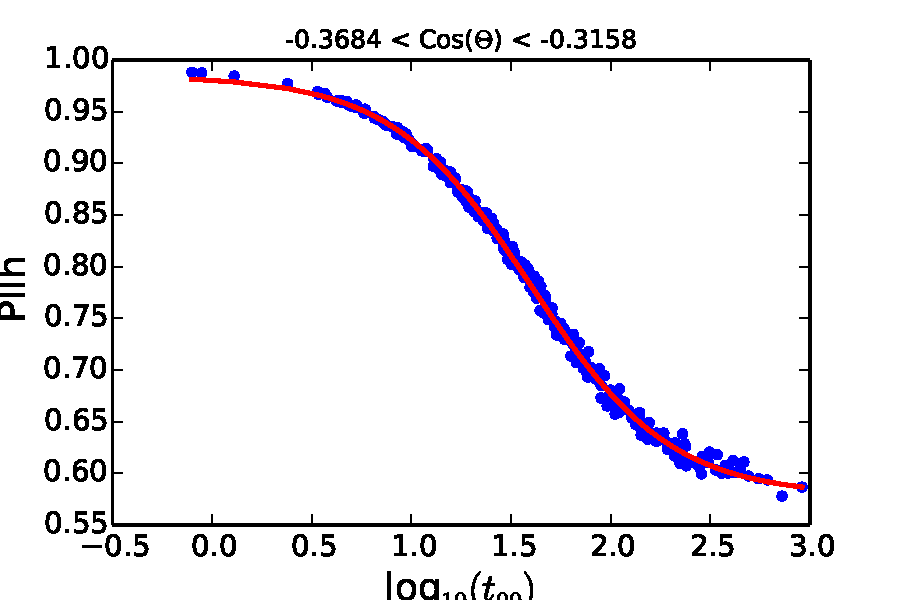
\includegraphics[width=\textwidth]{fig/Pllhparam.pdf}
% \caption{The probability of neutrino events to pass the cut on the test
% statistic and the dependency on the logarithm of the $t_{90}$ value for a
% certain cosinus bin. The red line represents the parameterization.}
% \label{fig:Pllhparam}
%  \end{minipage}
%  \begin{minipage}{0.5\textwidth}
%  \captionsetup{width=.9\textwidth}
%   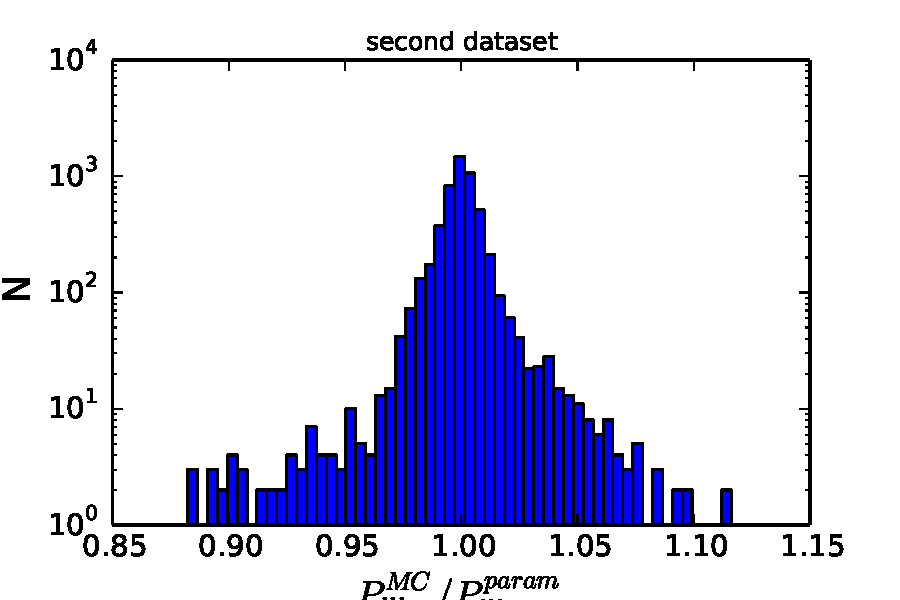
\includegraphics[width=\textwidth]{fig/Pllhparam_quality.pdf}
% \caption{Using a second dataset, a histogram of the ratio between the calculated
% and parametrized values is shown. Most GRBs fall within 5\% derivation while
% some outliers differ up to 12\%.\\}
%  \end{minipage}
% \end{figure}



The parameterization of $P_\text{llh}$ is more complicated than
$P_{3.5^\circ}$. The test statistic depends not only on properties of the 
simulated neutrino events like the zenith angle
% and thus the zenith angle
but on the time window 
between two neutrinos and, therefore, on $t_{90}$. The data is split 
into 180 cosinus bins
and the probability is fitted against the logarithm of the drawn $t_{90}$ (Eq.
\ref{eq:t90dist} and \ref{eq:t90earth}) value for each bin. The amount of 180 
bins is a compromise between precision and needed computational power. The 
probability changes rapidly near the pole requiring a high 
number of bins. In return, many simulated GRBs are needed to facilitate a good 
parameterization representing various GRBs per bin and $t_{90}$ value.

\begin{figure}[h]
 \centering
 \captionsetup{width=0.85\textwidth}
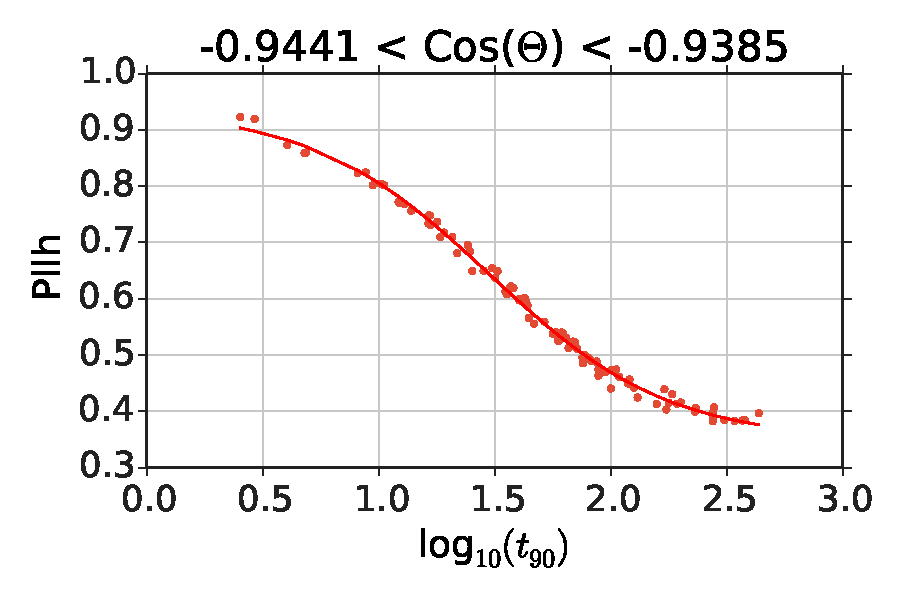
\includegraphics[width=0.6\textwidth]{fig/Pllh_example_g2_bdt.pdf}

\caption{The probability for a doublet to pass 
the cut on the likelihood (Eq. 
\ref{eq:alert-llh}) vs the logarithm of 
$t_{90}$. As an example, the cosinus bin of $-0.9441 < \cos \theta_\text{GRB} 
< -0.9385$ is shown. The red dots represent values calculated according to Eq. 
\ref{eq:Pllh} for drawn GRBs. The red line is a fit to these values. 
\label{fig:Pllh_example_g2_bdt}}
\end{figure}

An example based on a dataset for the IC86-BDT season and a spectral index of 
$\gamma=2$ is shown in Figure
\ref{fig:Pllh_example_g2_bdt} displaying individual calculated probabilities of 
GRBs as red dots and a fit to these points as a function of the logarithm of 
$t_{90}$. The fit is based on Eq. \ref{eq:Ptanh}. Such a fit is done for each 
bin in $\cos \theta_\text{GRB}$ and for each season - $\gamma$ combination in 
turn. Due to the large number of plots only an example is displayed.

The quality of the parameterization can be judged by examining Figure 
\ref{fig:Pllhparam_bdt_gamma2_quality}. The parameterization was applied to a 
second dataset for which the probability was calculated according to 
\ref{eq:Pllh} for all events within the zenith band. The ratio of calculated 
and parametrized values are displayed in the histogram. Both the root mean 
square with $0.006$ and the maximum deviation with about 3 
percentage points are satisfactory small. 

%proof that outliers average out???
%where do they lie??? which GRBs???
\begin{figure}[h]
\centering
 \captionsetup{width=.85\textwidth}
%  \captionsetup{margin=0pt}
\subfloat[Probability to pass 
likelihood cut.\label{fig:Pllhparam_bdt_gamma2_quality}]{%
 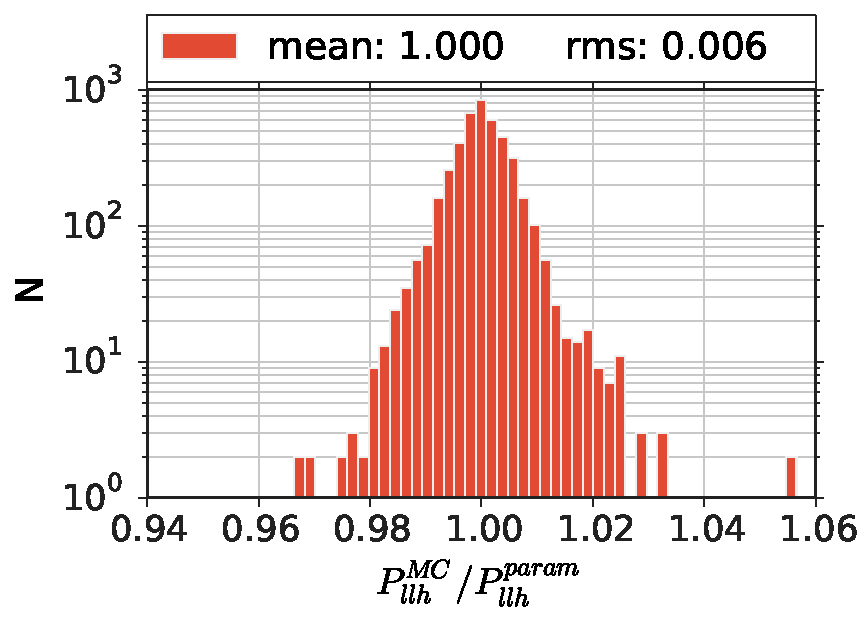
\includegraphics[width=0.45\textwidth]{fig/Pllhparam_bdt_gamma2_quality.pdf}}
 \subfloat[Probability for a GRB to be within Swift FoV. 
\label{fig:PonSparam_bdt_gamma2_quality}]{%
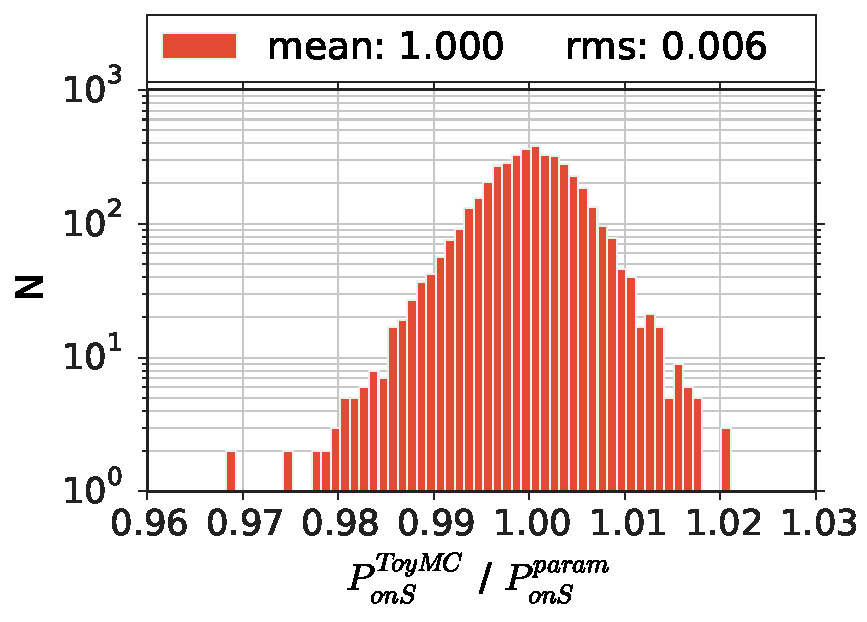
\includegraphics[width=0.45\textwidth]{fig/PonSparam_bdt_gamma2_quality.pdf}}
\caption{Season IC86-BDT: Using a second set of simulated GRBs, a histogram 
of the ratio between the calculated probabilities and the parametrized values 
is shown. The maximum deviation 
is of about 2 percentage points.}
\end{figure}


\paragraph{P$_\text{onS}$}$\;$\\
The Optical Follow-Up program calculates the weighted mean direction from all
events contributing to a multiplet using the Cramer Rao error as weights. For a 
source to be detectable
with Swift, its
direction must be within 0.5 degrees of the true source direction. The
probability $P_\text{onS}$ for two events to point back to the source well
enough is given by
the ratio of the sum over the event weight products fulfilling the condition
and the sum over all event weight products:
\begin{equation}
P_\text{onS} = \frac{\sum_i \sum_{j=i+1} w_i \cdot w_j |
\Psi_{\text{weighted mean}}(i, j) - \Psi_{GRB} \leq 0.5^{\circ} \; | \;
\lambda(i, j)
\leq \lambda_\text{cut} \; | \; \Delta \Psi(i, j) \leq 3.5^{\circ}}{\sum_i
\sum_{j=i+1} w_i \cdot w_j \; | \; \lambda(i, j)
\leq \lambda_\text{cut} \; | \; \Delta \Psi(i, j) \leq 3.5^{\circ}} 
\end{equation}
Only events passing the conditions $\Delta \Psi(i,j) \leq 3.5^\circ$ and 
$\lambda(i, j) \leq \lambda_\text{cut}$ are considered.
The parametrization is performed using the methods used and described for 
$P_\text{llh}$ leading to a similar quality as can be judged with the help of 
Figure 
\ref{fig:PonSparam_bdt_gamma2_quality}.

\paragraph{Alert Probability}$\;$\\
The probabilities described in this section until now are conditional and can 
be 
combined via multiplication according to the Base Theorem and the probability 
that two neutrinos are detected, trigger the Swift Follow-Up and that the 
source is within Swifts FoV is
\begin{equation}
 P_\text{Alert} = P_{2\nu} \cdot P_D \cdot P_\text{llh} \cdot P_\text{onS}.
\end{equation}
$P_\text{onS}$ can be set to one if only the probability to have a Swift
alert is of interest.

Given these parameterizations, a big number of usually around five 
million GRBs are thrown to create a sample representing the complete redshift 
and luminosity range.

%more detail? plot?


\subsubsection{Probability to Detect a GRB}
The previous section described a simplified case of only two neutrinos. 
However, if $\mu$ neutrinos are expected per GRB there is a chance to see more 
than two neutrinos. There are two trigger conditions for a Swift alert. 
Usually, one doublet is 
detected and passes the Swift cut on the OFU test statistic as 
well. However, there is the 
possibility of a 'higher multiplet' as well which we define as an alert of at 
least three neutrinos.

In both cases the number of possible 
doublets and the probability of them to be detected needs to be calculated. If 
$N$ neutrinos are detected, the first neutrino can be part of a doublet with 
$N-1$ partners, while the second neutrino can combine with $N-2$ partners. The 
general formula describing the number of possible combinations is the Gaussian 
Sum Formula
\begin{equation}
 d = 1 + 2 + ... + (x-1) + x= \frac{x^2 + x}{2}.
\end{equation}
Two neutrinos are needed to form a doublet, leading to the substitution $N = 
x-1$. The number of possible doublets is then 
\begin{equation}
 d = \frac{N^2 - N}{2}.
\end{equation}
with each doublet having a probability $P_D$ to pass the time window and 
angular separation cuts. The probability for this to happen $k$ out of $d$ 
times is given by the binomial distribution
\begin{equation}
 P_\text{bin} ( k, d(N), P_D) =  \binom{d}{k} \cdot P_{D}^k \cdot 
(1 - P_{D})^{d-k} = \binom{0.5 (N^2 - N)}{k} \cdot P_{D}^k \cdot 
(1 - P_{D})^{0.5(N^2 -N) -k}
\end{equation}

The correct probability to see exactly one doublet to is determined by 
multiplying the probability to see $N$ neutrinos and the probability of these 
$N$ 
neutrinos to form exactly one doublet for all $N \geq 2$
\begin{equation}
 P_\text{1 Doublet} = \sum_{N=2}^{N_\text{max}} P_\text{Poisson}(N, 
\mu) \cdot P_\text{bin} (1, d(N), P_D)
\end{equation}
$N_\text{max}$ is chosen to achieve a precision in the order of $10^{-6}$.
The probability that one doublet passes the likelihood cut as well is given by
\begin{equation}
 P_\text{1 Swift Doublet} = P_\text{1 Doublet} \cdot P_\text{llh}
\end{equation}

The second channel is triggered when at least three neutrinos 
result in at least two doublets.
\begin{equation}
 P_\text{Multiplet} = \sum_{n=3}^{n_\text{max}} P_\text{Poisson}(n, 
\mu) \cdot [1 - P_\text{bin} (0, d(n), P_D) - P_\text{bin} (1, 
d(n), P_D)]
\end{equation}

These definitions can be used to calculate the probability to detect a specific 
GRB. Generating $N_\text{gen} = 5\cdot10^6$ GRBs, the number of GRBs that are 
expected to be detected
in a specific channel is the sum over all probabilities, e.g. for higher 
multiplets
\begin{equation}
 N_\text{GRB} / yr = \sum_{i=0}^{N_\text{gen}} P_{\text{multiplet},i} \cdot 
\frac{N_\text{GRB, yr}}{N_\text{GRB, gen}}
\end{equation}
The ratio at the end is necessary to renormalize the result to the expected 
number of 
GRBs per year $N_\text{GRB, yr}$.

This concludes the description of the Toy Monte Carlo to calculate the expected 
number of expected signal alerts for different spectra and GRB models. The 
following section describes how to use the background and signal expectations 
 to calculate a test statistic. It will be used to draw limits on the 
contribution of transients to the HESE flux.
